\chapter{HASIL DAN PEMBAHASAN}
\section{Contoh Penyajian Gambar}
Gambar~\ref{fig:kurva} memperlihatkan contoh kurva $y=x^2$ yang dibuat sendiri menggunakan \texttt{TikZ}. Gambar ini merupakan ilustrasi mandiri, bukan reproduksi dari publikasi lain. Apabila gambar diadaptasi dari sumber luar, sumber aslinya wajib disebutkan dalam keterangan gambar dan daftar pustaka.
\begin{figure}[htbp]
\centering
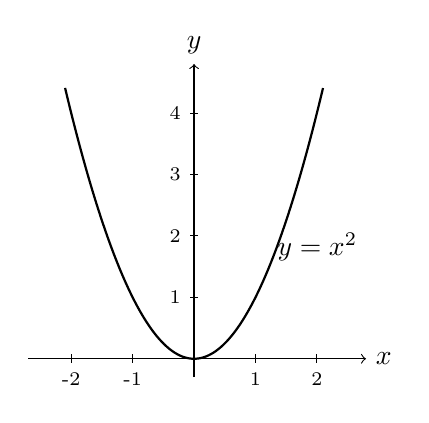
\begin{tikzpicture}[scale=0.78]
  \draw[->] (-2.7,0) -- (2.8,0) node[right] {$x$};
  \draw[->] (0,-0.3) -- (0,4.8) node[above] {$y$};
  \draw[thick,domain=-2.1:2.1,samples=100,smooth] plot (\x,{\x*\x});
  \node[above right] at (1.2,1.44) {$y=x^2$};
  \foreach \x in {-2,-1,1,2} {\draw (\x,0.07)--(\x,-0.07) node[below] {\scriptsize \x};}
  \foreach \y in {1,2,3,4} {\draw (0.06,\y)--(-0.06,\y) node[left] {\scriptsize \y};}
\end{tikzpicture}
\caption{Ilustrasi kurva fungsi kuadrat (sumber: dibuat oleh penulis)}
\label{fig:kurva}
\end{figure}

\section{Contoh Penyajian Tabel dan Rujukan}
Tabel~\ref{tab:contoh} memuat nilai fungsi yang diperoleh secara analitik. Data pada tabel merupakan contoh perhitungan, bukan hasil penelitian. Pembahasan metode perhitungan dan kestabilan numerik dapat merujuk pada sumber akademik yang relevan, misalnya \cite{higham2002}.
\begin{table}[htbp]
\centering
\caption{Nilai fungsi $f(x)=x^2$ pada beberapa titik (sumber: perhitungan penulis)}
\label{tab:contoh}
\begin{tabular}{cc}
\toprule
$x$ & $f(x)$ \\
\midrule
0 & 0 \\
1 & 1 \\
2 & 4 \\
\bottomrule
\end{tabular}
\end{table}

\section{Pembahasan}
Jelaskan makna temuan, hubungan dengan teori, perbandingan dengan literatur, serta batasan yang relevan. Pastikan setiap gambar dan tabel dirujuk dari teks; jangan hanya menampilkannya tanpa analisis.
